\chapter{Observables qui commutent, phases d’énergie et précession du spin}

\lectureoverview{Nous commençons par le sens qualitatif de l’incertitude. Deux observables ne peuvent avoir simultanément des valeurs bien définies que si elles possèdent une base complète commune de vecteurs propres, ce qui équivaut à la commutation de leurs opérateurs. Nous récapitulons ensuite l’évolution unitaire et l’équation de Schr\"odinger, comparons les commutateurs aux crochets de Poisson classiques, résolvons l’équation dépendant du temps dans la base d’énergie, puis appliquons le résultat à un spin dans un champ magnétique. Le calcul final donne la précession des valeurs moyennes du spin, les deux niveaux d’énergie d’un Hamiltonien de spin général, ainsi que la distinction entre une valeur moyenne transverse et un photon d’énergie égale à la moitié de l’écart entre les niveaux.}

Le spin à deux états reste notre système quantique le plus simple. Un espace de Hilbert à trois états serait la prochaine possibilité abstraite la plus simple ; deux spins ont déjà quatre états de base orthogonaux. Nous n’allons pas encore composer deux spins, même si cette étape est proche et fera intervenir l’intrication. Commençons par achever le problème d’un seul spin et asseoir plus solidement les idées d’incertitude et d’évolution temporelle.

\section{Quand deux grandeurs peuvent-elles être simultanément bien définies ?}

Une bonne mesure est répétable. Si l’on mesure une observable et que l’on obtient la valeur \(l\), une répétition immédiate doit donner le même résultat. La première mesure doit donc laisser le système, au moins momentanément, dans un état propre de l’opérateur correspondant :
\begin{equation}
L\ket{l}=l\ket{l}.
\end{equation}
Cette caractérisation opérationnelle suffit à faire apparaître l’origine qualitative de l’incertitude.

Supposons que deux observables \(L\) et \(M\) puissent être mesurées simultanément. Une mesure conjointe doit laisser bien définies les deux valeurs obtenues. Les états possibles après la mesure doivent donc être des vecteurs propres simultanés des deux opérateurs. Dans le cadre de dimension finie utilisé ici, nous pouvons choisir un ensemble orthonormé complet \(\{\ket{i}\}\) vérifiant
\begin{equation}
L\ket{i}=l_i\ket{i},
\qquad
M\ket{i}=m_i\ket{i}.
\label{eq:l5-common-eigenvectors}
\end{equation}

\begin{remark}
Le terme \emph{base} désignera une base orthonormée complète. L’algèbre linéaire admet des bases non orthogonales, mais la convention orthonormée est particulièrement naturelle pour les états quantiques. En présence de valeurs propres dégénérées, il reste une liberté à l’intérieur de chaque sous-espace propre ; on peut y choisir les vecteurs propres de façon à obtenir un ensemble orthonormé.
\end{remark}

\begin{theorem}
Deux observables hermitiennes de dimension finie sont mesurables simultanément si et seulement si elles admettent une base propre commune complète, ce qui équivaut à leur commutation.
\end{theorem}

Le sens direct découle immédiatement de l’équation~\eqref{eq:l5-common-eigenvectors}. En appliquant les opérateurs dans un ordre, on obtient
\begin{align}
ML\ket{i}
&=M\bigl(l_i\ket{i}\bigr)\\
&=l_i m_i\ket{i},
\end{align}
tandis que, dans l’ordre inverse, on obtient
\begin{align}
LM\ket{i}
&=L\bigl(m_i\ket{i}\bigr)\\
&=m_i l_i\ket{i}.
\end{align}
Les valeurs propres sont des nombres ordinaires, donc \(l_i m_i=m_i l_i\). Ainsi, \(ML\) et \(LM\) agissent de la même manière sur chaque vecteur de la base, et donc sur chaque état :
\begin{equation}
[L,M]\equiv LM-ML=0.
\label{eq:l5-commuting-condition}
\end{equation}

\begin{figure}[htbp]\centering
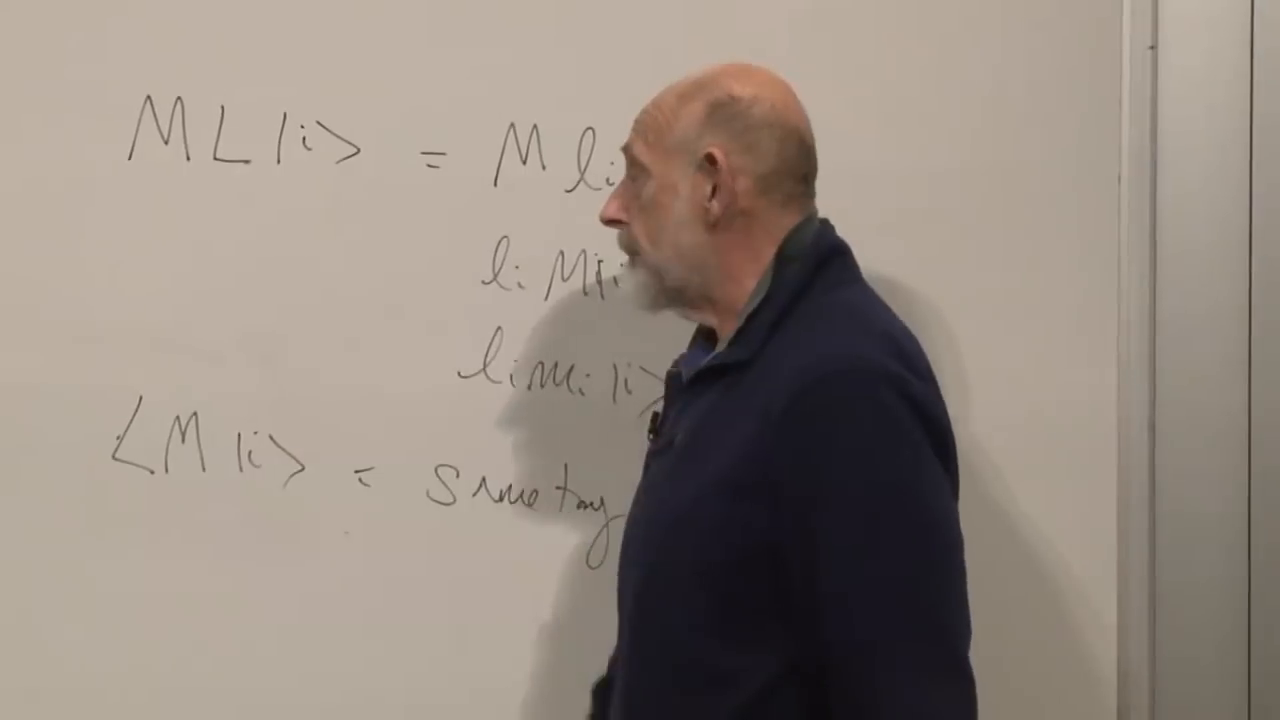
\includegraphics[width=0.86\textwidth]{lecture_05_figure_02.png}\caption{Les opérateurs commutent lorsque \(LM-ML=[L,M]=0\).}\lectureframe{00:10:30}\end{figure}

La réciproque est également vraie : des opérateurs hermitiens qui commutent peuvent être diagonalisés simultanément. Si l’un des opérateurs possède un sous-espace propre dégénéré, l’autre préserve ce sous-espace et peut y être diagonalisé. En procédant de même dans chacun des sous-espaces propres, on obtient une base propre commune complète.

Les opérateurs de Pauli fournissent le premier contre-exemple important. Aucun couple parmi \(\sigma_x,\sigma_y,\sigma_z\) ne commute. Les états propres de \(\sigma_z\) sont les états haut et bas, tandis que ceux de \(\sigma_x\) sont les états droite et gauche. On peut préparer un état où l’une ou l’autre composante est parfaitement déterminée et répéter sa mesure, mais on ne peut pas préparer simultanément un état où les deux composantes sont parfaitement déterminées. Voilà l’incertitude avant même d’introduire une quelconque inégalité numérique.

Nous quantifierons plus tard la manière dont les incertitudes de deux observables qui ne commutent pas se contraignent mutuellement. Aucune relation numérique d’incertitude n’est démontrée ici. Le point présent précède l’inégalité : la non-commutation empêche un état d’attribuer simultanément des valeurs bien définies aux deux grandeurs.

\begin{classroomqa}\audiencequestion{Pourquoi une mesure simultanée exige-t-elle des vecteurs propres communs ?}\lecturerresponse{Une mesure répétable laisse l’état avec une valeur mesurée bien définie, ce qui signifie qu’il est dans un état propre de l’opérateur mesuré. Si deux valeurs sont obtenues simultanément et que les mesures de ces deux valeurs restent répétables, l’état qui en résulte doit être un état propre des deux opérateurs. L’ensemble complet des résultats conjoints fournit donc une base propre commune.}\end{classroomqa}

\begin{classroomqa}\audiencequestion{Cela concerne-t-il deux particules différentes ?}\lecturerresponse{Pas nécessairement, puisque \(\sigma_x\) et \(\sigma_z\) agissent déjà sur un seul spin. En revanche, pour deux sous-systèmes distincts, les observables qui agissent sur des facteurs différents commutent : \(A\otimes I\) commute avec \(I\otimes B\). C’est pourquoi on peut mesurer simultanément une composante d’un spin et une composante d’un autre. La composition de tels systèmes nous conduira plus tard à l’intrication.}\end{classroomqa}

\section{Évolution unitaire et générateur}

Il a fallu bien plus de temps à la mécanique quantique qu’à la mécanique classique pour définir un état, mais une fois l’espace des états établi, la règle d’évolution est compacte. Soit
\begin{equation}
\ket{\psi(t)}=U(t)\ket{\psi(0)}.
\label{eq:l5-propagator}
\end{equation}
L’évolution temporelle doit préserver la distinguabilité. Plus encore, elle préserve tous les produits scalaires. Pour une base orthonormée,
\begin{equation}
\bra{j}U^\dagger(t)U(t)\ket{i}=\delta_{ji},
\end{equation}
et donc
\begin{equation}
U^\dagger(t)U(t)=I.
\label{eq:l5-unitarity}
\end{equation}
L’opérateur d’évolution est unitaire.

À temps écoulé nul, \(U(0)=I\). La continuité implique alors qu’une évolution pendant un petit intervalle de temps \(\epsilon\) ne diffère que légèrement de l’identité. Dans les unités où \(\hbar=1\), écrivons
\begin{equation}
U(\epsilon)=I-i\epsilon H+O(\epsilon^2),
\qquad
U^\dagger(\epsilon)=I+i\epsilon H^\dagger+O(\epsilon^2).
\end{equation}
En substituant cette expression dans l’équation~\eqref{eq:l5-unitarity}, on obtient
\begin{equation}
H^\dagger=H.
\end{equation}
Le générateur de l’évolution temporelle est hermitien, et constitue donc une observable. C’est le Hamiltonien.

L’application du propagateur infinitésimal à un état donne
\begin{equation}
\ket{\psi(\epsilon)}
=\ket{\psi(0)}-i\epsilon H\ket{\psi(0)}+O(\epsilon^2).
\end{equation}
En réarrangeant, on obtient le quotient de différences écrit au tableau :
\begin{equation}
\frac{\ket{\psi(\epsilon)}-\ket{\psi(0)}}{\epsilon}
=-iH\ket{\psi(0)}+O(\epsilon).
\end{equation}

\begin{figure}[htbp]\centering
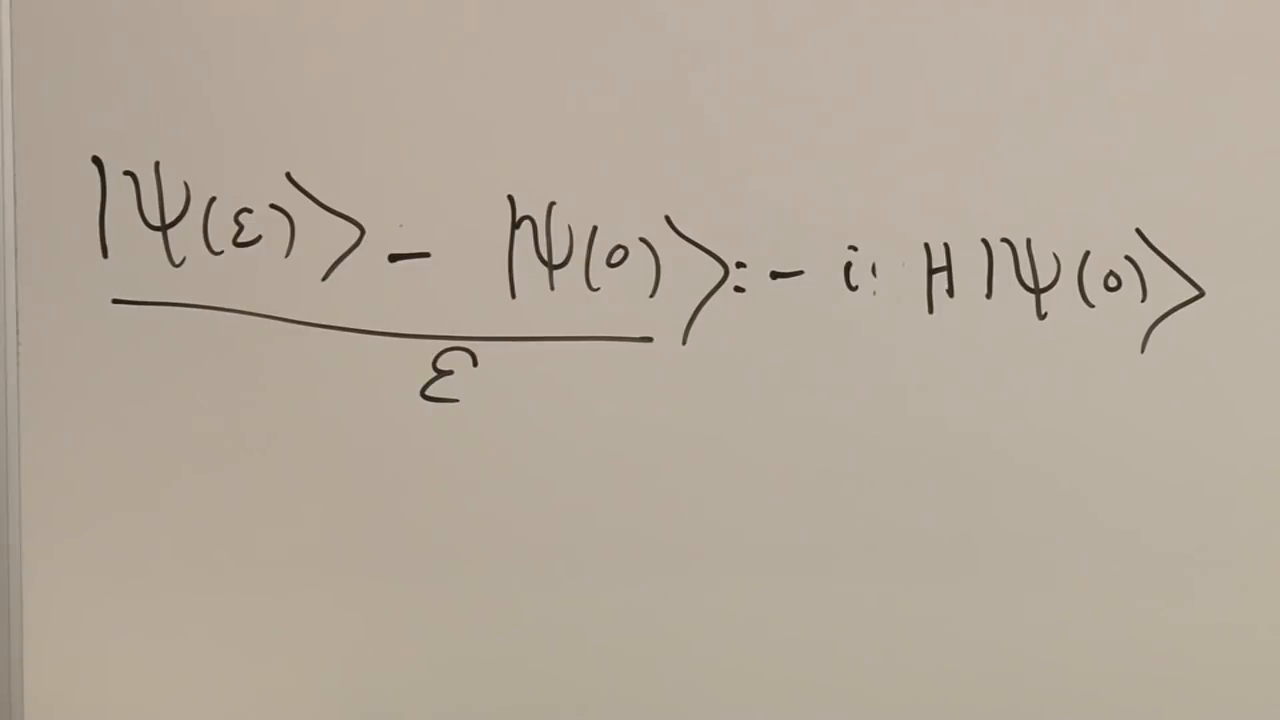
\includegraphics[width=0.86\textwidth]{lecture_05_figure_03.png}\caption{Mise à jour infinitésimale écrite sous la forme d’un quotient de différences.}\lectureframe{00:23:33}\end{figure}

En prenant \(\epsilon\to0\), on obtient l’équation de Schr\"odinger dépendant du temps :
\begin{equation}
\frac{d}{dt}\ket{\psi(t)}=-iH\ket{\psi(t)}.
\label{eq:l5-schrodinger}
\end{equation}
En rétablissant les constantes, on trouve \(i\hbar\,d\ket{\psi}/dt=H\ket{\psi}\).

L’équation originale de Schr\"odinger portait sur la fonction d’onde d’une particule en mouvement. On a autrefois appelé l’énoncé opératoriel ci-dessus l’équation de Schr\"odinger généralisée, car elle s’applique aussi bien à un spin, à un système à trois états, à deux spins ou à un système de complexité arbitraire. L’adjectif a largement disparu : c’est désormais simplement la forme générale de l’équation.

L’équation~\eqref{eq:l5-schrodinger} détermine l’évolution de l’état lorsque le système reste isolé. Cela ne signifie pas que chaque résultat expérimental soit déterminé. Un état quantique fixe les probabilités des différentes mesures possibles, et l’équation les fait évoluer par l’intermédiaire des amplitudes. En général, une mesure modifie l’état et interrompt cette évolution isolée.

\begin{classroomqa}\audiencequestion{Toute mesure perturbe-t-elle le système ?}\lecturerresponse{En général, oui, mais il existe un cas particulier important. Si l’état est déjà un état propre de l’observable, une mesure idéale et répétable peut en confirmer la valeur sans modifier cet état. En général, il n’est pas possible de mesurer une observable arbitraire sans perturber d’autres propriétés incompatibles.}\end{classroomqa}

\section{Énergie et équation indépendante du temps}

Comme \(H\) est hermitien, ses valeurs propres sont réelles et ses vecteurs propres peuvent être choisis de façon à former une base orthonormée complète :
\begin{equation}
H\ket{E_i}=E_i\ket{E_i}.
\label{eq:l5-time-independent}
\end{equation}
C’est la forme indépendante du temps de l’équation de Schr\"odinger. Il s’agit d’un problème aux valeurs propres, et non d’une équation du mouvement : on cherche les valeurs d’énergie possibles du système et les états dans lesquels ces valeurs sont parfaitement déterminées.

Le spectre dépend du système. Les états liés d’un atome et l’oscillateur harmonique ont des niveaux d’énergie dénombrables. Une particule non liée peut avoir un spectre continu. L’énergie peut se mesurer de nombreuses façons ; en principe, même une mesure de masse suffisamment précise pourrait faire appel à \(E=mc^2\), bien que ce soit rarement la méthode pratique. Un système réel possède déjà son Hamiltonien : le physicien ne le fixe pas, mais cherche à le découvrir. Une fois cet opérateur connu, trouver ses valeurs propres et ses vecteurs propres est une tâche mathématique.

Ajouter une constante \(cI\) à \(H\) décale chaque énergie de \(c\). Cela multiplie l’état entier par une phase commune \(e^{-ict}\), qui ne modifie ni les probabilités ni les valeurs moyennes. Dans la dynamique considérée ici, seules les différences d’énergie ont un effet.

\section{Évolution des valeurs moyennes}

L’expression usuelle \emph{valeur moyenne} désigne une moyenne statistique. Pour une observable \(L\),
\begin{equation}
\expect{L}(t)=\bra{\psi(t)}L\ket{\psi(t)}.
\end{equation}
À ce stade, seuls les vecteurs d’état dépendent du temps. En dérivant les deux membres et en utilisant l’équation~\eqref{eq:l5-schrodinger} ainsi que son conjugué hermitien,
\begin{equation}
\frac{d}{dt}\ket{\psi}=-iH\ket{\psi},
\qquad
\frac{d}{dt}\bra{\psi}=i\bra{\psi}H,
\end{equation}
on obtient
\begin{align}
\frac{d}{dt}\expect{L}
&=i\bra{\psi}HL\ket{\psi}
  -i\bra{\psi}LH\ket{\psi}\\
&=-i\expect{[L,H]}.
\label{eq:l5-expectation-motion}
\end{align}

\begin{figure}[htbp]\centering
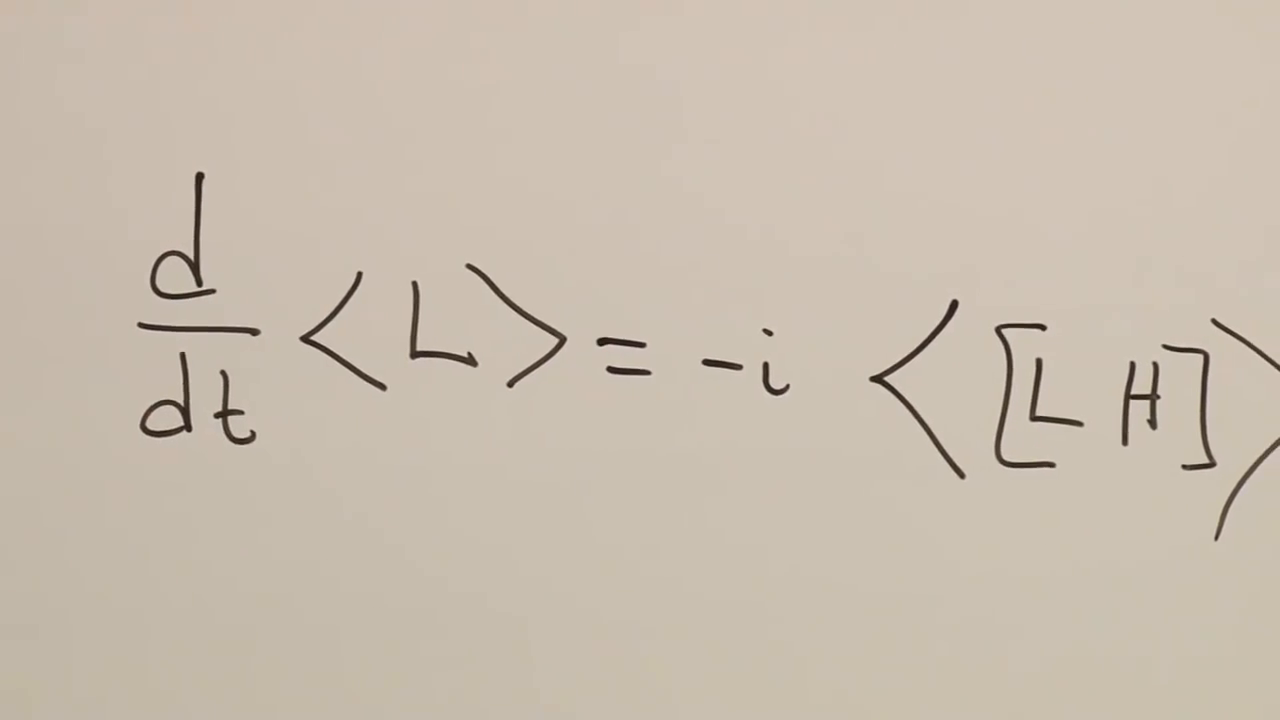
\includegraphics[width=0.86\textwidth]{lecture_05_figure_04.png}\caption{Équation d’évolution de la valeur moyenne sous forme commutateur.}\lectureframe{00:35:35}\end{figure}

Le facteur \(i\) ne compromet pas le caractère réel de \(\expect{L}\). Pour des opérateurs hermitiens \(L\) et \(H\), le commutateur est anti-hermitien :
\begin{equation}
[L,H]^\dagger=-[L,H].
\end{equation}
Sa valeur moyenne est donc purement imaginaire ; multipliée par \(-i\), elle donne une dérivée réelle.

On utilise parfois la notation abrégée
\begin{equation}
\dot L=-i[L,H].
\end{equation}
À ce stade, il faut la lire comme une abréviation de l’équation~\eqref{eq:l5-expectation-motion}, qui porte sur les valeurs moyennes. Nous étudierons plus tard un changement complet de représentation, dans lequel les opérateurs eux-mêmes dépendent du temps.

\subsection{Algèbre des commutateurs}

Les commutateurs sont antisymétriques :
\begin{equation}
[A,B]=-[B,A].
\end{equation}
Ils obéissent également à une règle du produit analogue à la règle de Leibniz pour les dérivées :
\begin{equation}
[AB,C]=A[B,C]+[A,C]B.
\label{eq:l5-product-rule}
\end{equation}
Pour le vérifier, conservons l’ordre de chaque facteur :
\begin{align}
A[B,C]+[A,C]B
&=A(BC-CB)\\
&\quad +(AC-CA)B\\
&=ABC-ACB\\
&\quad +ACB-CAB\\
&=ABC-CAB\\
&=[AB,C].
\end{align}

\begin{figure}[htbp]\centering
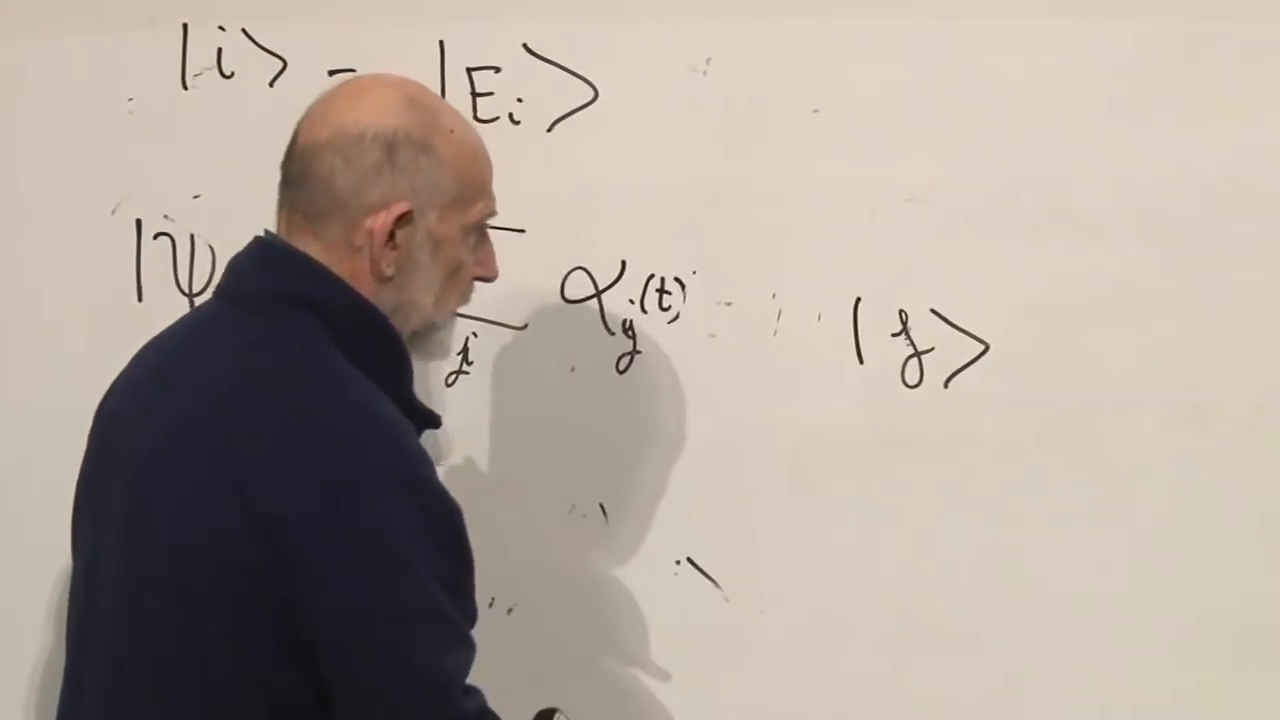
\includegraphics[width=0.86\textwidth]{lecture_05_figure_05.png}\caption{Vérification de la règle du produit pour les commutateurs par développement des deux membres.}\lectureframe{00:43:10}\end{figure}

\begin{classroomqa}\audiencequestion{Le membre de droite de la règle du produit ne compte-t-il pas par inadvertance deux fois le membre de gauche ?}\lecturerresponse{Non. Après développement, \(ABC\) et \(-CAB\) sont les deux termes voulus. Les deux termes ajoutés sont \(-ACB\) et \(+ACB\) ; ils se compensent exactement. La répétition apparente est le terme provisoire nécessaire pour factoriser l’expression des deux façons requises.}\end{classroomqa}

La même antisymétrie et la même règle du produit s’appliquent aux crochets de Poisson classiques. Cette ressemblance structurelle n’est pas fortuite. La correspondance classique est
\begin{equation}
\{A,B\}
\quad\longleftrightarrow\quad
\frac{1}{i\hbar}[A,B]
=-\frac{i}{\hbar}[A,B].
\label{eq:l5-poisson-correspondence}
\end{equation}
Dans les unités où \(\hbar=1\), l’équation classique
\begin{equation}
\frac{dL}{dt}=\{L,H\}
\end{equation}
a la même forme que l’équation~\eqref{eq:l5-expectation-motion}. Dans les unités macroscopiques usuelles, \(\hbar\) est minuscule et les commutateurs deviennent négligeables dans la limite classique appropriée. C’est le contrôle essentiel qui identifie le générateur quantique \(H\) au Hamiltonien de la mécanique classique.

Le facteur \(\hbar\) est nécessaire pour des raisons dimensionnelles. Un crochet de Poisson fait intervenir des dérivées par rapport aux coordonnées et aux moments conjugués, tandis qu’un commutateur d’opérateurs est directement construit à partir de produits. La constante de Planck assure la conversion entre ces dimensions.

Posons \(L=H\). Comme tout opérateur commute avec lui-même,
\begin{equation}
\frac{d}{dt}\expect{H}
=-i\expect{[H,H]}=0.
\end{equation}
Pour les Hamiltoniens indépendants du temps considérés ici, l’énergie moyenne se conserve. On peut établir un énoncé plus fort concernant toute la distribution de l’énergie, mais la valeur moyenne suffit pour l’instant.

\begin{classroomqa}\audiencequestion{Que désigne \(L\) dans ces équations ? S’agit-il du moment cinétique ?}\lecturerresponse{Ici, \(L\) est un opérateur linéaire hermitien générique, donc une observable quelconque. Il peut s’agir d’une composante du spin, d’une position ou même de \(H\). La lettre a été choisie pour \emph{opérateur linéaire} ; il ne faut pas y voir le moment cinétique, sauf si cette interprétation est indiquée séparément.}\end{classroomqa}

\begin{classroomqa}\audiencequestion{Pourquoi le facteur \(i\) ne donne-t-il pas une dérivée imaginaire à une valeur moyenne réelle ?}\lecturerresponse{Le commutateur de deux opérateurs hermitiens est anti-hermitien ; sa valeur moyenne est donc imaginaire. Le calcul des matrices de Pauli ci-dessous le montre concrètement : leurs commutateurs contiennent un facteur explicite \(2i\), qui se simplifie avec le \(-i\) dans l’équation du mouvement.}\end{classroomqa}

\section{Résoudre l’équation de Schr\"odinger dans la base d’énergie}

Supposons que le problème aux valeurs propres de l’énergie soit résolu. Développons un état arbitraire dans la base d’énergie fixe :
\begin{equation}
\ket{\psi(t)}=\sum_j\alpha_j(t)\ket{E_j}.
\label{eq:l5-energy-expansion}
\end{equation}
Dans cette représentation, les vecteurs de base ne changent pas ; toute la dépendance temporelle se trouve dans les coefficients. En substituant l’équation~\eqref{eq:l5-energy-expansion} dans l’équation~\eqref{eq:l5-schrodinger}, on obtient
\begin{align}
\sum_j\dot\alpha_j(t)\ket{E_j}
&=-i\sum_j\alpha_j(t)H\ket{E_j}\\
&=-i\sum_j E_j\alpha_j(t)\ket{E_j}.
\end{align}
L’unicité du développement dans une base implique, pour chaque \(j\) fixé,
\begin{equation}
\dot\alpha_j(t)=-iE_j\alpha_j(t),
\qquad\text{no sum on \(j\)}.
\end{equation}
La solution est
\begin{equation}
\alpha_j(t)=\alpha_j(0)e^{-iE_jt}.
\label{eq:l5-energy-phase}
\end{equation}

\begin{figure}[htbp]\centering
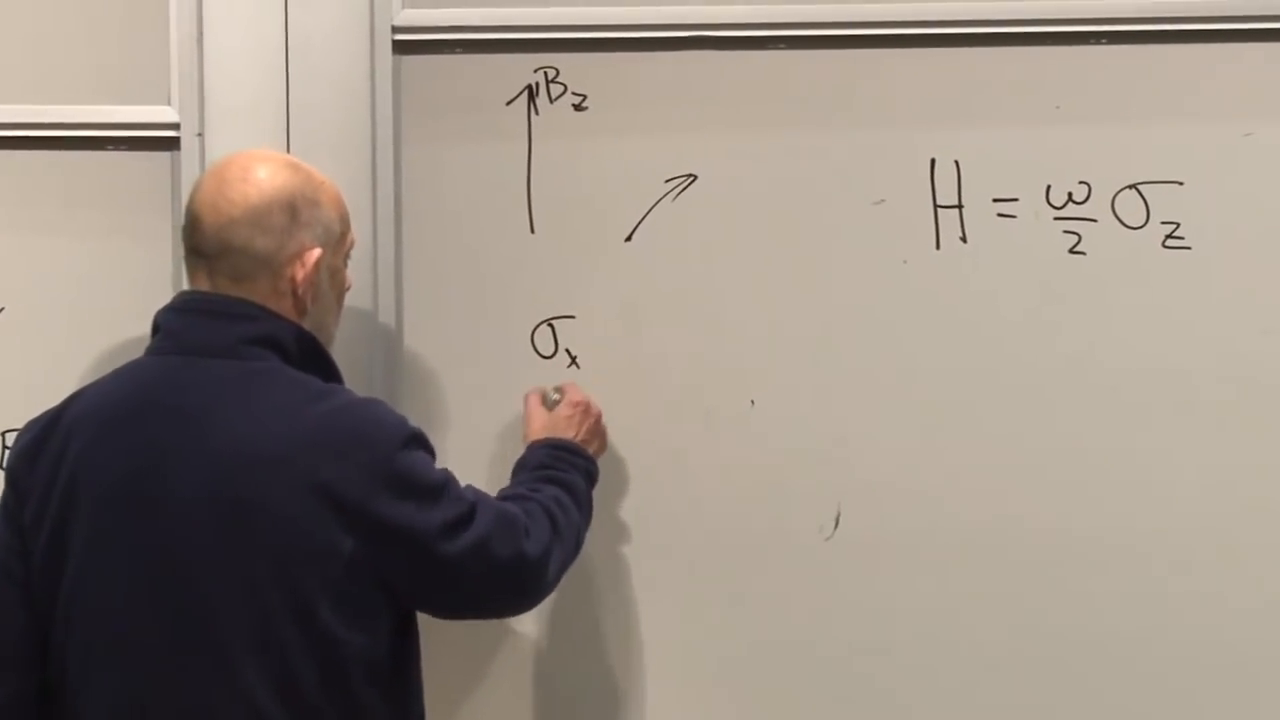
\includegraphics[width=0.86\textwidth]{lecture_05_figure_06.png}\caption{Chaque coefficient dans la base d’énergie satisfait sa propre équation de phase exponentielle.}\lectureframe{01:03:25}\end{figure}

La solution générale est donc
\begin{equation}
\ket{\psi(t)}
=\sum_j\alpha_j(0)e^{-iE_jt}\ket{E_j}.
\label{eq:l5-general-solution}
\end{equation}
En rétablissant les unités, on remplace \(E_jt\) par \(E_jt/\hbar\). Le module de chaque coefficient reste constant :
\begin{equation}
|\alpha_j(t)|=|\alpha_j(0)|.
\end{equation}
L’évolution temporelle modifie les phases relatives. Un état propre d’énergie unique n’acquiert qu’une phase commune ; ses probabilités de mesure sont donc indépendantes du temps.

On peut maintenant écrire explicitement la valeur moyenne de \(L\). Définissons ses éléments de matrice dans la base d’énergie par
\begin{equation}
L_{kj}=\bra{E_k}L\ket{E_j}.
\end{equation}
On a alors
\begin{align}
\expect{L}(t)
&=\sum_{k,j}
\alpha_k^*(0)\alpha_j(0)
e^{i(E_k-E_j)t}
L_{kj}.
\label{eq:l5-heisenberg-matrix}
\end{align}

\begin{figure}[htbp]\centering
\includegraphics[width=0.86\textwidth]{lecture_05_figure_07.png}\caption{Formule matricielle dans la base d’énergie : chaque élément est accompagné d’une phase à la fréquence de transition correspondante.}\lectureframe{01:10:45}\end{figure}

Les termes diagonaux \(k=j\) sont constants. Un élément de matrice non diagonal oscille à la fréquence correspondant à la différence d’énergie \(E_k-E_j\). Dans le récit historique présenté ici, Heisenberg a reconnu cette organisation matricielle avant que la dérivation moderne par les vecteurs d’état n’existe ; la notation de Dirac en a ensuite rendu le sens limpide.

\begin{classroomqa}\audiencequestion{Le module des coefficients \(\alpha_j\) reste-t-il constant ?}\lecturerresponse{Oui. Chaque coefficient est multiplié par une phase complexe de module unité. Seules les phases relatives changent ; elles permettent aux valeurs moyennes comportant des éléments de matrice non diagonaux de varier avec le temps.}\end{classroomqa}

\begin{classroomqa}\audiencequestion{Dans l’équation de Schr\"odinger, faut-il utiliser une dérivée partielle ou une dérivée totale ?}\lecturerresponse{Pour l’état abstrait \(\ket{\psi(t)}\) considéré ici, le temps est la seule variable explicitée ; les deux notations expriment donc la même chose. Plus tard, une fonction d’onde telle que \(\psi(x,t)\) dépendra à la fois de la position et du temps, et la notation avec une dérivée partielle sera alors naturelle.}\end{classroomqa}

\begin{classroomqa}\audiencequestion{La préservation de l’orthogonalité est-elle seulement une hypothèse empirique ?}\lecturerresponse{Elle est étayée par l’expérience, mais elle est aussi remarquablement rigide. Les tentatives de déformer la mécanique quantique unitaire tendent à détruire la positivité ou la conservation de la probabilité, la localité causale ou le traitement cohérent des systèmes composites. David Finkelstein décrivait les théories déformables comme soumises à un écoulement plastique et les théories rigides comme se fissurant de façon cassante. En ce sens, la mécanique quantique est cassante : de petites modifications arbitraires ne conduisent généralement pas à une théorie cohérente voisine.}\end{classroomqa}

\begin{classroomqa}\audiencequestion{Pourquoi les valeurs propres de l’énergie \(E_j\) sont-elles réelles ?}\lecturerresponse{L’unitarité implique que le générateur infinitésimal \(H\) est hermitien, et toute valeur propre d’un opérateur hermitien est réelle. On a donc la chaîne suivante : préservation de l’orthogonalité, unitarité, caractère hermitien de \(H\), puis réalité du spectre d’énergie.}\end{classroomqa}

\section{Un spin dans un champ magnétique}

Quel Hamiltonien faut-il attribuer à un spin isolé ? Un spin dans l’espace vide, sans interaction, n’a aucune direction privilégiée non triviale ; son Hamiltonien est donc proportionnel à l’identité et ne produit aucun mouvement observable. Un champ magnétique fournit à la fois une énergie d’interaction et un axe.

Plaçons le champ selon \(z\). Une particule chargée portant un spin possède un moment magnétique, et l’énergie dipolaire habituelle est proportionnelle à l’alignement de ce moment sur le champ. Regroupons l’intensité du champ, le moment magnétique, la convention de signe et \(\hbar\) dans une constante \(\omega\) :
\begin{equation}
H=\frac{\omega}{2}\sigma_z.
\label{eq:l5-z-hamiltonian}
\end{equation}
Le facteur \(1/2\) est commode, car les commutateurs de Pauli contiennent un facteur \(2\).

Il faut interpréter avec prudence l’image classique de la flèche. Un spin quantique ne possède pas de valeurs simultanément bien définies pour ses composantes \(x\), \(y\) et \(z\) ; aucune flèche ordinaire ne peut donc représenter toutes ses propriétés à la fois. L’objet tridimensionnel utile sera le vecteur des valeurs moyennes, et non le vecteur d’état à deux composantes lui-même.

\subsection{Commutateurs des matrices de Pauli}

Utilisons les représentations matricielles
\begin{equation}
\begin{aligned}
\sigma_x&=
\begin{pmatrix}0&1\\1&0\end{pmatrix},\\[0.4em]
\sigma_y&=
\begin{pmatrix}0&-i\\i&0\end{pmatrix},\\[0.4em]
\sigma_z&=
\begin{pmatrix}1&0\\0&-1\end{pmatrix}.
\end{aligned}
\end{equation}
Par exemple,
\begin{align}
[\sigma_z,\sigma_x]
&=
\begin{pmatrix}1&0\\0&-1\end{pmatrix}
\begin{pmatrix}0&1\\1&0\end{pmatrix}
-
\begin{pmatrix}0&1\\1&0\end{pmatrix}
\begin{pmatrix}1&0\\0&-1\end{pmatrix}\\
&=
\begin{pmatrix}0&1\\-1&0\end{pmatrix}
-
\begin{pmatrix}0&-1\\1&0\end{pmatrix}\\
&=2
\begin{pmatrix}0&1\\-1&0\end{pmatrix}
=2i\sigma_y.
\end{align}
Les relations cycliques sont
\begin{equation}
\begin{aligned}
[\sigma_z,\sigma_x]&=2i\sigma_y,\\
[\sigma_x,\sigma_y]&=2i\sigma_z,\\
[\sigma_y,\sigma_z]&=2i\sigma_x.
\end{aligned}
\label{eq:l5-pauli-commutators}
\end{equation}
Inverser l’ordre de l’un ou l’autre des opérateurs inverse le signe.

\begin{figure}[htbp]\centering
\includegraphics[width=0.86\textwidth]{lecture_05_figure_08.png}\caption{Les trois commutateurs de Pauli se referment cycliquement sur les matrices de Pauli elles-mêmes.}\lectureframe{01:33:30}\end{figure}

Ces relations ont la même structure cyclique que les crochets de Poisson classiques du moment cinétique. Elles se referment également sur les trois opérateurs initiaux, ce qui simplifie particulièrement les équations du mouvement.

\begin{classroomqa}\audiencequestion{Faut-il calculer les commutateurs à l’aide des crochets bra-ket ?}\lecturerresponse{Non. La multiplication des opérateurs se représente par la multiplication des matrices ; les matrices \(2\times2\) permettent donc un calcul direct commode. On pourrait aussi appliquer successivement les opérateurs aux états de base haut et bas et obtenir le même résultat.}\end{classroomqa}

\subsection{Précession des valeurs moyennes}

Appliquons l’équation~\eqref{eq:l5-expectation-motion} avec l’Hamiltonien de l’équation~\eqref{eq:l5-z-hamiltonian} :
\begin{align}
\frac{d}{dt}\expect{\sigma_x}
&=-i\frac{\omega}{2}\expect{[\sigma_x,\sigma_z]}
=-\omega\expect{\sigma_y},\\
\frac{d}{dt}\expect{\sigma_y}
&=-i\frac{\omega}{2}\expect{[\sigma_y,\sigma_z]}
=+\omega\expect{\sigma_x},\\
\frac{d}{dt}\expect{\sigma_z}
&=-i\frac{\omega}{2}\expect{[\sigma_z,\sigma_z]}
=0.
\label{eq:l5-spin-motion}
\end{align}

\begin{figure}[htbp]\centering
\begin{minipage}[c]{0.62\textwidth}\centering
\includegraphics[width=\textwidth]{lecture_05_figure_09.png}\end{minipage}\hfill
\begin{minipage}[c]{0.31\textwidth}\centering
\begin{tikzpicture}[scale=0.78,>=Latex]
  \draw[->,thick] (0,0) -- (0,3.0) node[above] {\(z\parallel\bm B\)};
  \draw[dashed] (0,1.8) ellipse (1.45 and 0.42);
  \draw[->,very thick] (0,0) -- (1.05,1.8)
    node[right] {\(\expect{\bm\sigma}\)};
  \draw[->,thick] (1.38,1.67)
    arc[start angle=-12,end angle=245,x radius=1.45,y radius=0.42];
\end{tikzpicture}\end{minipage}\caption{Les équations au tableau et leur conséquence géométrique : les valeurs moyennes transverses tournent, tandis que la composante parallèle au champ reste constante. La flèche représente les trois valeurs moyennes, et non un spin classique caché.}\lectureframe{01:35:28}\end{figure}

Les deux premières équations décrivent un mouvement circulaire dans le plan transverse :
\begin{align}
\expect{\sigma_x}(t)
&=\expect{\sigma_x}(0)\cos\omega t
-\expect{\sigma_y}(0)\sin\omega t,\\
\expect{\sigma_y}(t)
&=\expect{\sigma_x}(0)\sin\omega t
+\expect{\sigma_y}(0)\cos\omega t.
\end{align}
Pendant ce temps, \(\expect{\sigma_z}\) reste constant. Le vecteur des valeurs moyennes précesse donc autour de l’axe du champ magnétique à la fréquence angulaire \(\omega\).

Dans ce calcul en représentation de Schr\"odinger, les opérateurs sont des matrices fixes. C’est l’état qui évolue, et donc les valeurs moyennes qui décrivent le mouvement gyroscopique familier.

\begin{classroomqa}\audiencequestion{Comment un espace d’états à deux dimensions peut-il donner lieu à une image de précession en trois dimensions ?}\lecturerresponse{Le vecteur d’état possède deux composantes complexes, à un facteur de normalisation et à une phase globale près. Le vecteur réel représenté est plutôt \(\bigl(\expect{\sigma_x},\expect{\sigma_y},\expect{\sigma_z}\bigr)\). Ces valeurs moyennes sont déterminées par l’état et forment la représentation par le vecteur de Bloch, mais elles ne sont pas le vecteur d’état lui-même.}\end{classroomqa}

\section{Hamiltonien le plus général pour un spin unique}

Toute matrice hermitienne \(2\times2\) peut se développer sous la forme
\begin{equation}
H=aI+b_x\sigma_x+b_y\sigma_y+b_z\sigma_z,
\end{equation}
avec des coefficients réels. Le terme proportionnel à l’identité ne fait que modifier la phase globale. Les trois autres coefficients peuvent être considérés comme les composantes d’un vecteur. Notons \(\omega/2\) son module et \(\bm n\) sa direction, représentée par un vecteur unitaire ; l’Hamiltonien non trivial devient
\begin{equation}
H=\frac{\omega}{2}\,\bm\sigma\cdot\bm n,
\qquad
\bm\sigma\cdot\bm n
=n_x\sigma_x+n_y\sigma_y+n_z\sigma_z.
\label{eq:l5-general-spin-h}
\end{equation}
Si \(\bm B=B\bm n\), alors \(\bm n\) indique la direction du champ, tandis que \(\omega\) en représente le module, auquel est incorporé le couplage magnétique. C’est \(\bm n\), et non \(\omega\), qui indique l’orientation.

L’équation du mouvement prend la forme compacte
\begin{equation}
\frac{d}{dt}\expect{\bm\sigma}
=\omega\,\bm n\times\expect{\bm\sigma}.
\end{equation}
La composante selon \(\bm n\) commute avec \(H\) et reste constante ; les composantes perpendiculaires précessent autour de \(\bm n\).

\begin{classroomqa}\audiencequestion{Pourquoi est-ce la forme correcte de l’Hamiltonien ?}\lecturerresponse{Il n’existe que quatre matrices hermitiennes \(2\times2\) indépendantes : \(I,\sigma_x,\sigma_y,\sigma_z\). Le terme proportionnel à l’identité ne produit aucun mouvement observable du spin ; tout Hamiltonien non trivial indépendant du temps pour un spin unique est donc une combinaison linéaire réelle des trois matrices de Pauli. Un champ magnétique regroupe ces trois coefficients en un module et une direction.}\end{classroomqa}

\begin{classroomqa}\audiencequestion{Que représente exactement \(\omega\) ?}\lecturerresponse{C’est un scalaire proportionnel au produit du module du champ par le moment magnétique, avec les constantes conventionnelles incorporées. Il fixe à la fois la vitesse de précession et l’écart entre les niveaux d’énergie. Le vecteur unitaire \(\bm n\) précise la direction du champ.}\end{classroomqa}

\subsection{Les deux niveaux d’énergie}

En écrivant l’équation~\eqref{eq:l5-general-spin-h} sous forme matricielle, on obtient
\begin{equation}
\bm\sigma\cdot\bm n
=
\begin{pmatrix}
n_z & n_x-in_y\\
n_x+in_y & -n_z
\end{pmatrix}.
\end{equation}
Notons ses valeurs propres \(\lambda_1,\lambda_2\). Sa trace est nulle :
\begin{equation}
\lambda_1+\lambda_2=0.
\end{equation}
Pour un vecteur unitaire \(n_x^2+n_y^2+n_z^2=1\), son déterminant vaut
\begin{align}
\lambda_1\lambda_2
&=\det(\bm\sigma\cdot\bm n)\\
&=-n_z^2-(n_x-in_y)(n_x+in_y)\\
&=-(n_x^2+n_y^2+n_z^2)\\
&=-1.
\end{align}
Les deux valeurs propres sont donc
\begin{equation}
\lambda_\pm=\pm1.
\end{equation}

\begin{figure}[htbp]\centering
\includegraphics[width=0.86\textwidth]{lecture_05_figure_10.png}\caption{La trace et le déterminant fixent les valeurs propres de \(\bm\sigma\cdot\bm n\) à \(+1\) et \(-1\).}\lectureframe{01:59:20}\end{figure}

Par conséquent,
\begin{equation}
E_\pm=\pm\frac{\omega}{2},
\qquad
\Delta E=E_+-E_-=\omega.
\label{eq:l5-spin-gap}
\end{equation}
La direction du champ modifie les vecteurs propres d’énergie, mais pas ces deux valeurs propres.

\begin{classroomqa}\audiencequestion{Quel est le lien entre l’émission d’un photon et ces niveaux ?}\lecturerresponse{Lorsque le champ de rayonnement est inclus, le niveau de spin supérieur peut se désexciter vers le niveau inférieur en émettant un photon d’énergie \(\Delta E=\omega\) dans la convention \(\hbar=1\) utilisée ici. Le spin bascule alors entre les deux orientations opposées le long de l’axe du champ. Le calcul de précession négligeait ce faible couplage radiatif ; un spin peut donc précesser de nombreuses fois avant d’émettre.}\end{classroomqa}

\begin{classroomqa}\audiencequestion{Pourquoi le champ magnétique est-il traité comme un nombre plutôt que comme un opérateur quantique ?}\lecturerresponse{On traite provisoirement l’aimant comme un appareil classique massif, dont les fluctuations et le recul sont négligeables. Une description complète l’inclurait dans un système quantique plus vaste. En pratique, la séparation entre système et appareil se justifie lorsque celui-ci possède de nombreux degrés de liberté et que ses variables pertinentes fluctuent si peu que l’électron ne peut pas les modifier sensiblement.}\end{classroomqa}

\begin{classroomqa}\audiencequestion{Les équations de précession régulière décrivent-elles chaque essai individuel ?}\lecturerresponse{Elles décrivent les valeurs moyennes, donc les moyennes calculées sur des essais préparés de manière identique. Les mesures individuelles restent probabilistes. Des échantillons répétés tendent à approcher la moyenne théorique, mais la théorie des probabilités ne garantit pas un résultat exact pour toute séquence finie, pas plus qu’un million de lancers de pièce ne garantit exactement autant de piles que de faces.}\end{classroomqa}

\begin{classroomqa}\audiencequestion{Si le spin est orienté de côté, la transition émet-elle un demi-photon ?}\lecturerresponse{Non. Un état de spin orienté de côté est une superposition des deux états propres d’énergie. Dans le cas symétrique, il a une probabilité d’une moitié d’occuper le niveau supérieur et d’une moitié d’occuper le niveau inférieur. Il peut donc émettre un photon entier d’énergie \(\omega\), ou n’en émettre aucun. Son énergie moyenne émise peut être \(\omega/2\), mais aucun photon individuel ne porte la moitié de l’écart entre les niveaux.}\end{classroomqa}

Nous avons maintenant épuisé la dynamique non triviale indépendante du temps d’un spin unique. La même algèbre qui signalait d’abord l’incertitude engendre aussi son mouvement : les matrices de Pauli qui ne commutent pas transforment l’Hamiltonien en précession, tandis que la composante qui commute avec l’Hamiltonien se conserve. La complexité supplémentaire ne viendra pas d’un nouvel Hamiltonien pour un spin unique, mais d’un espace d’états plus vaste, où des systèmes indépendants pourront être composés et intriqués.
